\chapter{Results}\label{results}

The comparison between the $M_{VZ}^{T}$ distribution observed in data and the standard model
background prediction is used to test the existence of a new resonance decaying into VZ vector bosons.
No significant excess of events in data has been observed in this distribution, as shown in figures \ref{fig:fits3} and \ref{fig:fits4}.
We follow the modified frequentist prescription described in references \cite{CLs1,Junk:1999kv}(asymptotic CLs method). The limits are computed using an unbinned shape analysis. Systematic uncertainties are treated as nuisance parameters and profiled in the statistical interpretation using log-normal priors.

Upper limits at 95$\%$ confidence level (CL) are obtained
on the production cross section of a new resonance decaying to the
ZZ and WZ final state using the bulk graviton model and the $W'$ model to compute the signal efficiencies respectively, for each of the two categories in the analysis, high-purity and low-purity, under the narrow-width approximation assuming an integrated luminosity of 2.3 fb$^{-1}$. The resulting limits for different categories and the combination are shown in the figures \ref{fig:limits1} and \ref{fig:limits2}.


\begin{figure}[!ht]
\caption{ Observed and expected 95$\%$ CL upper limit on Bulk graviton production cross section times the branching fraction of $G_{bulk} \rightarrow  ZZ$ assuming an integrated luminosity of 2.3 fb$^{-1}$. The limit is obtained with the Asymptotic CLs technique. Top: (left) Expected limit for the HP category (right) Expected limit for the LP category. Bottom: Expected limits for the combination of both categories.}
\label{fig:limits1}
\begin{tabular}{cc}
  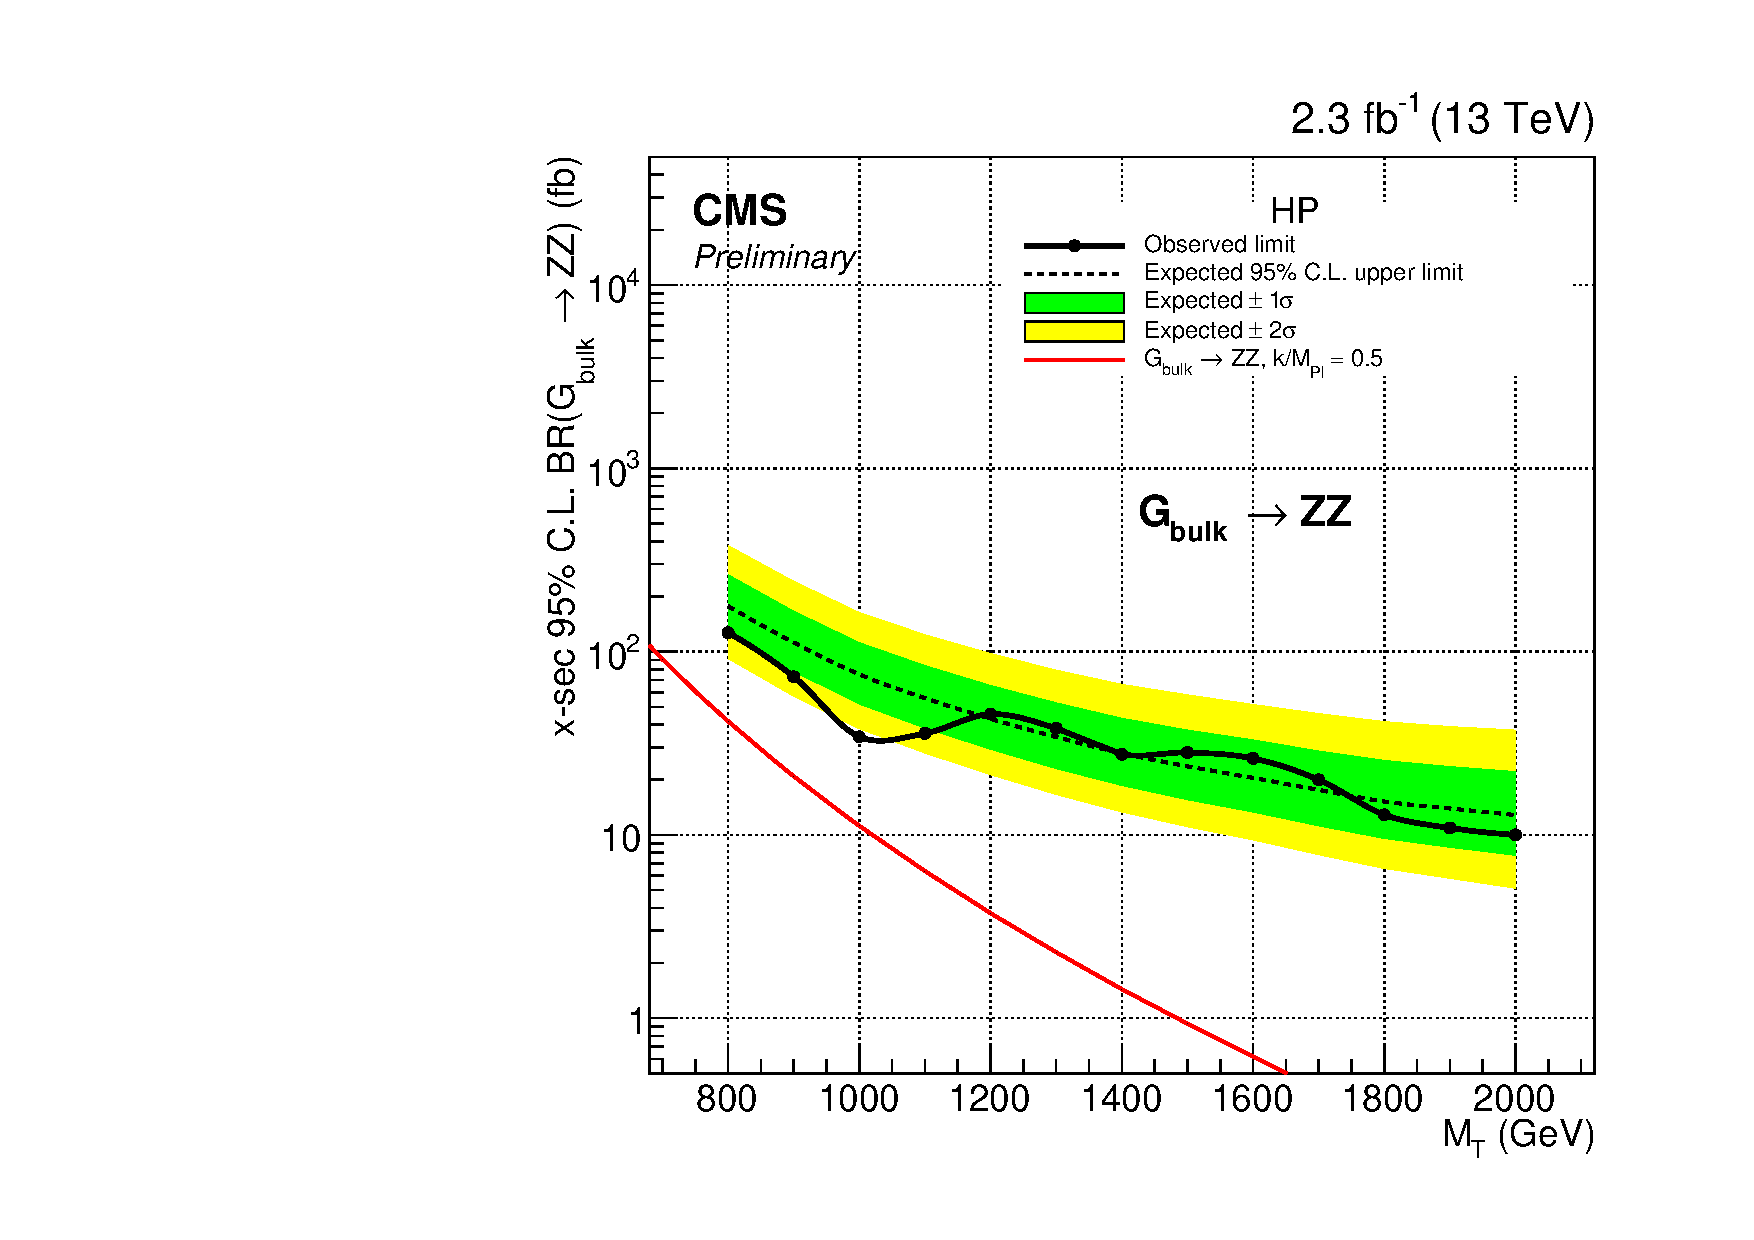
\includegraphics[width=200pt]{figuresARC/limits/limitBulkGHP.pdf} &
  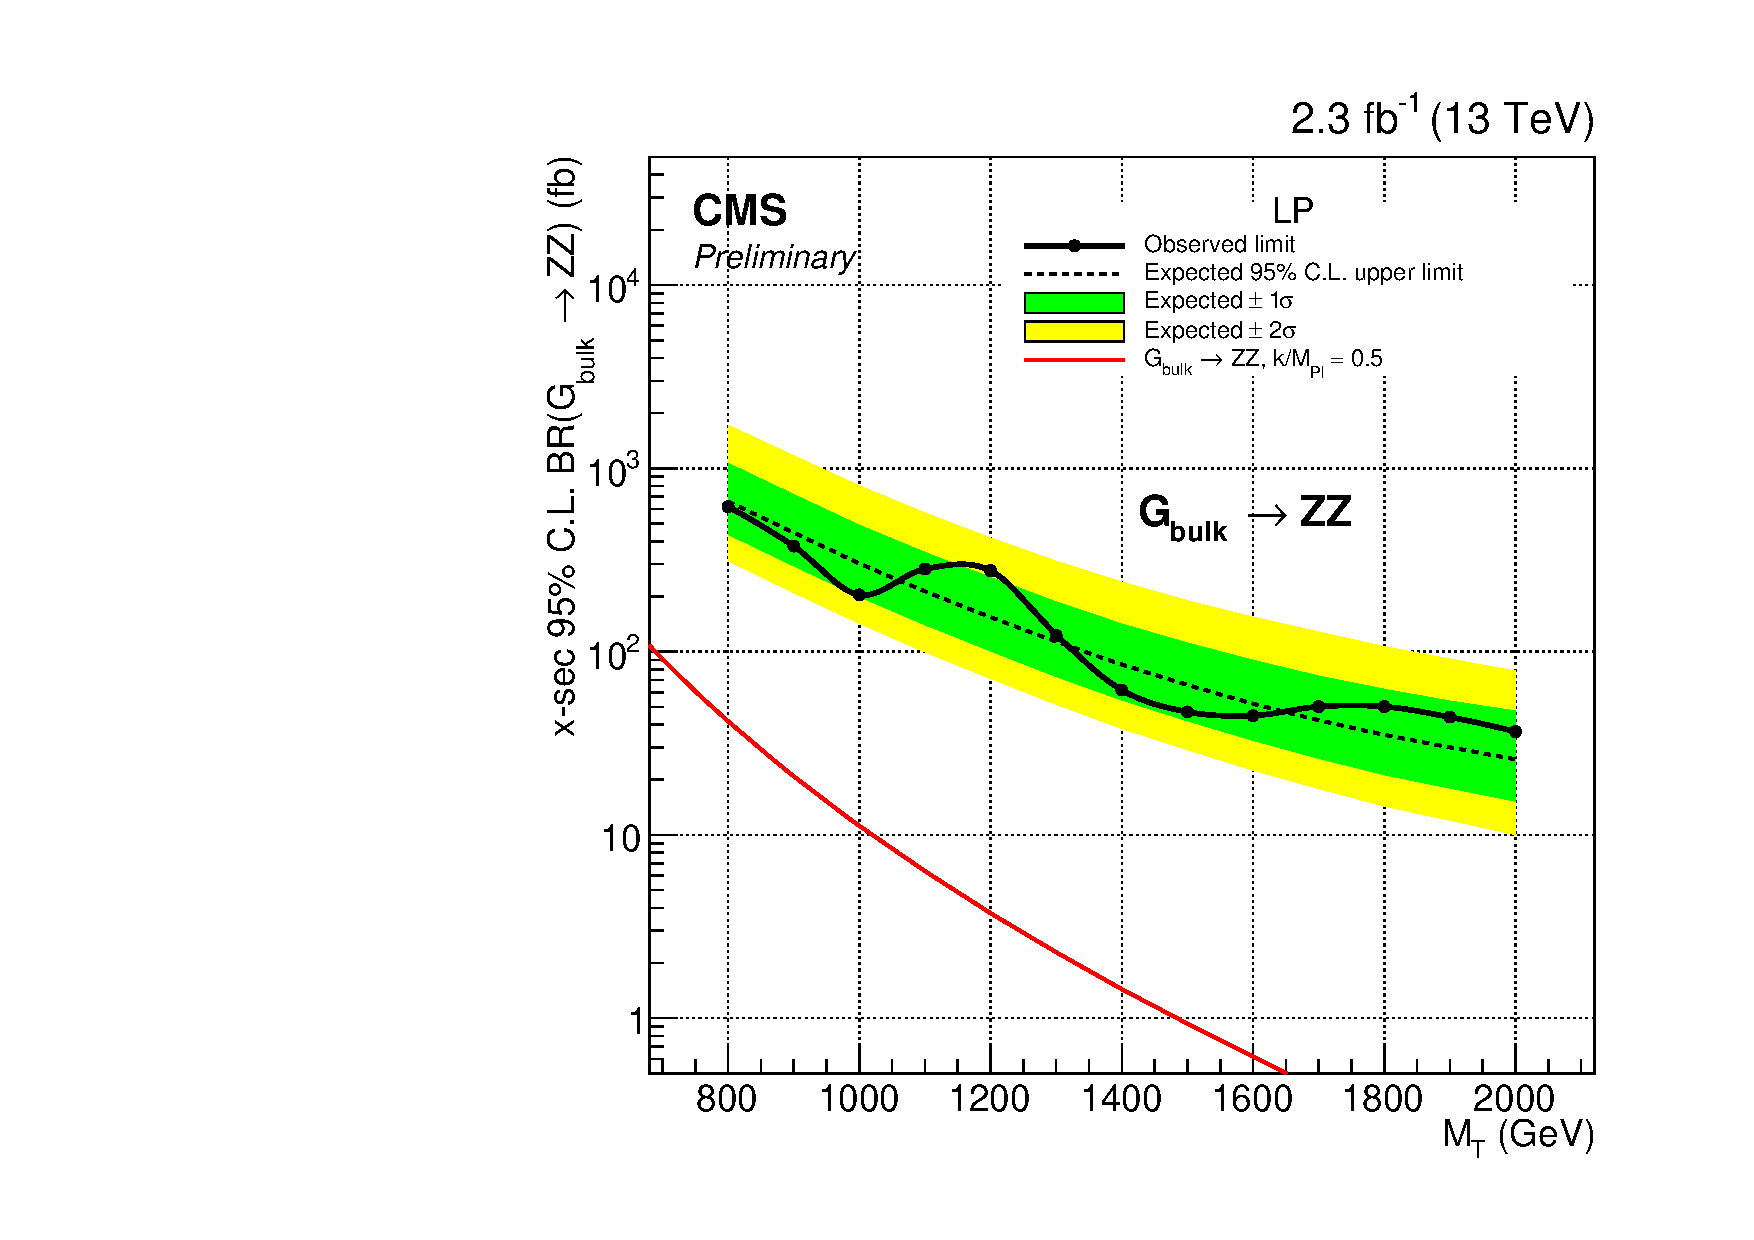
\includegraphics[width=200pt]{figuresARC/limits/limitBulkGLP.pdf}\\
\end{tabular}
\begin{center}
  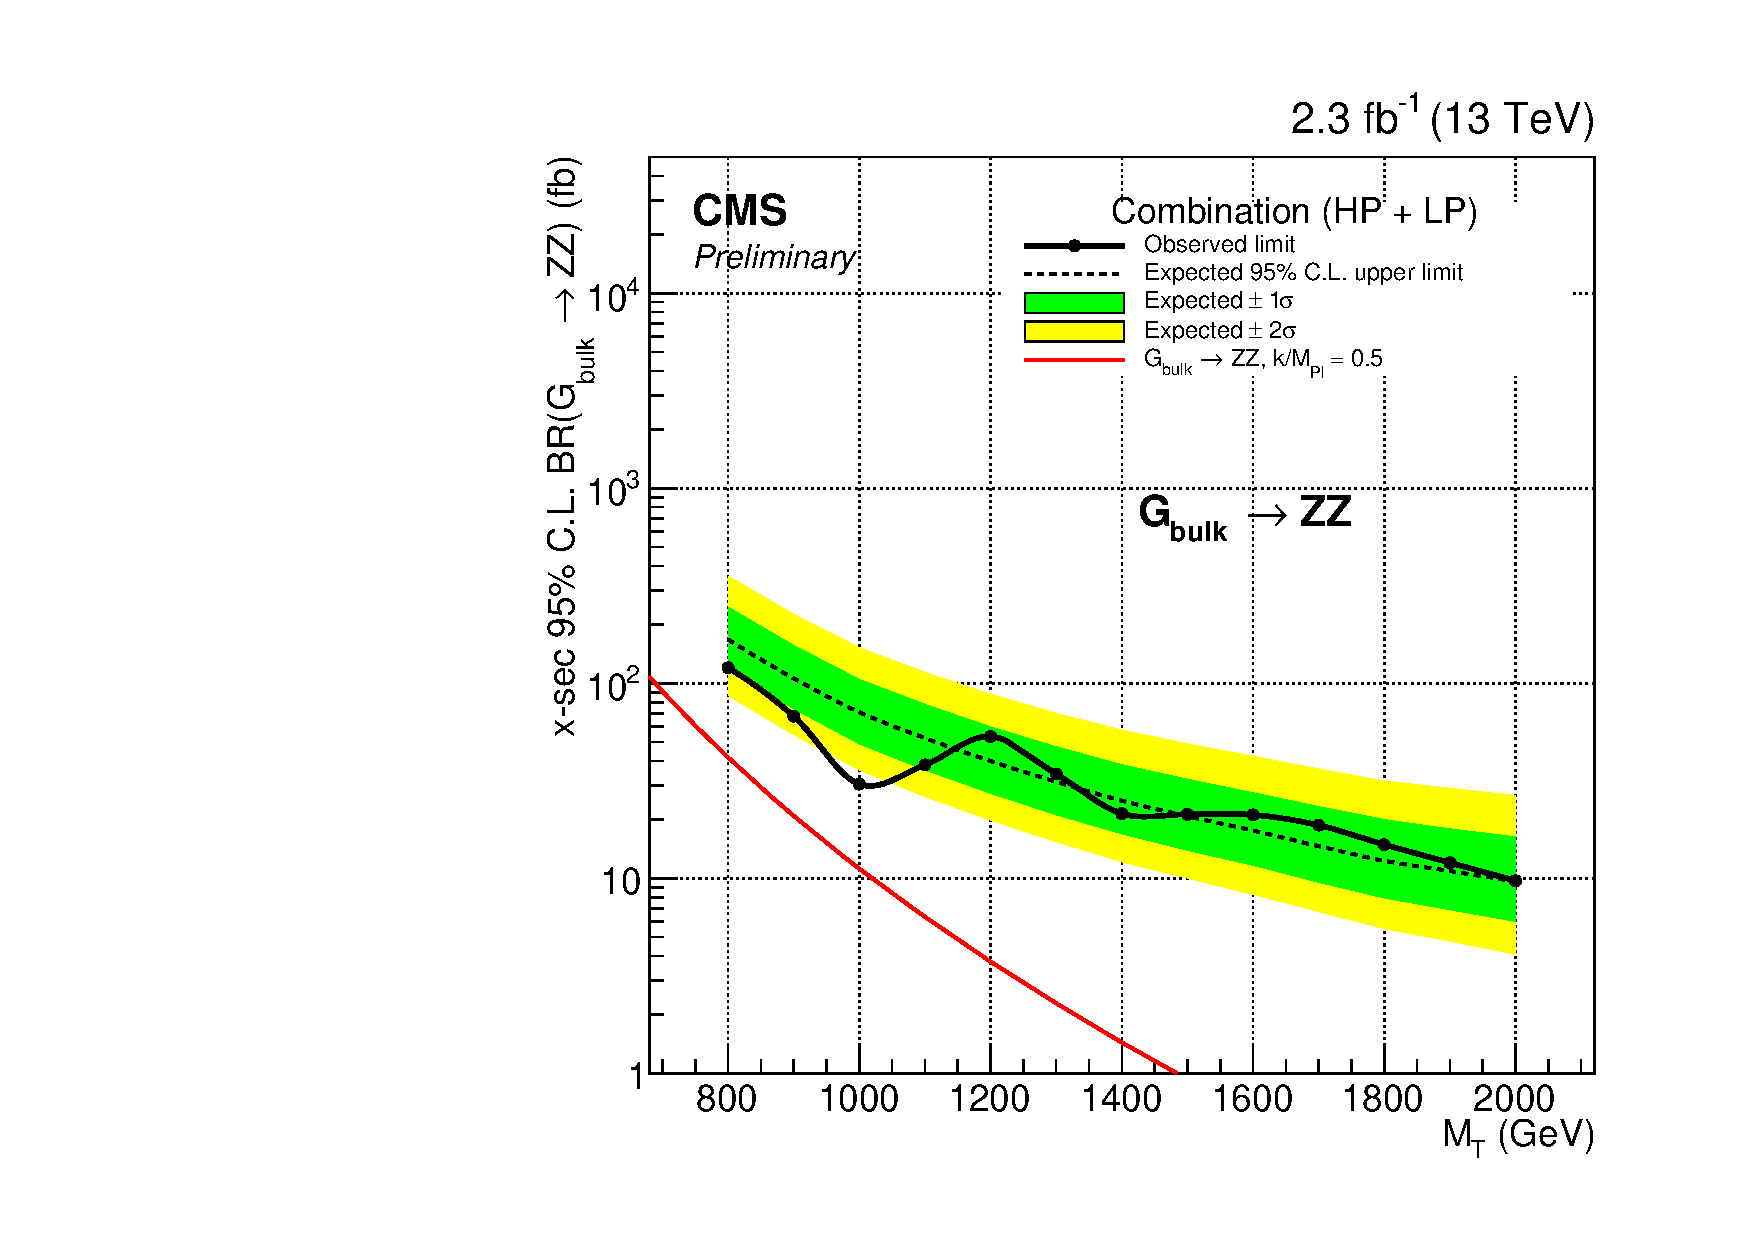
\includegraphics[width=250pt]{figuresARC/limits/limitBulkGNP.pdf}
\end{center}
\end{figure}

\begin{figure}[!ht]
\caption{ Observed and expected 95$\%$ CL upper limit on the $W'$ production cross section times the branching fraction of $G_{W'} \rightarrow  WZ$ assuming an integrated luminosity of 2.3 fb$^{-1}$. The limit is obtained with the Asymptotic CLs technique. Top: (left) Expected limit for the HP category (right) Expected limit for the LP category. Bottom: Expected limits for the combination of both categories.}
\begin{tabular}{cc}
  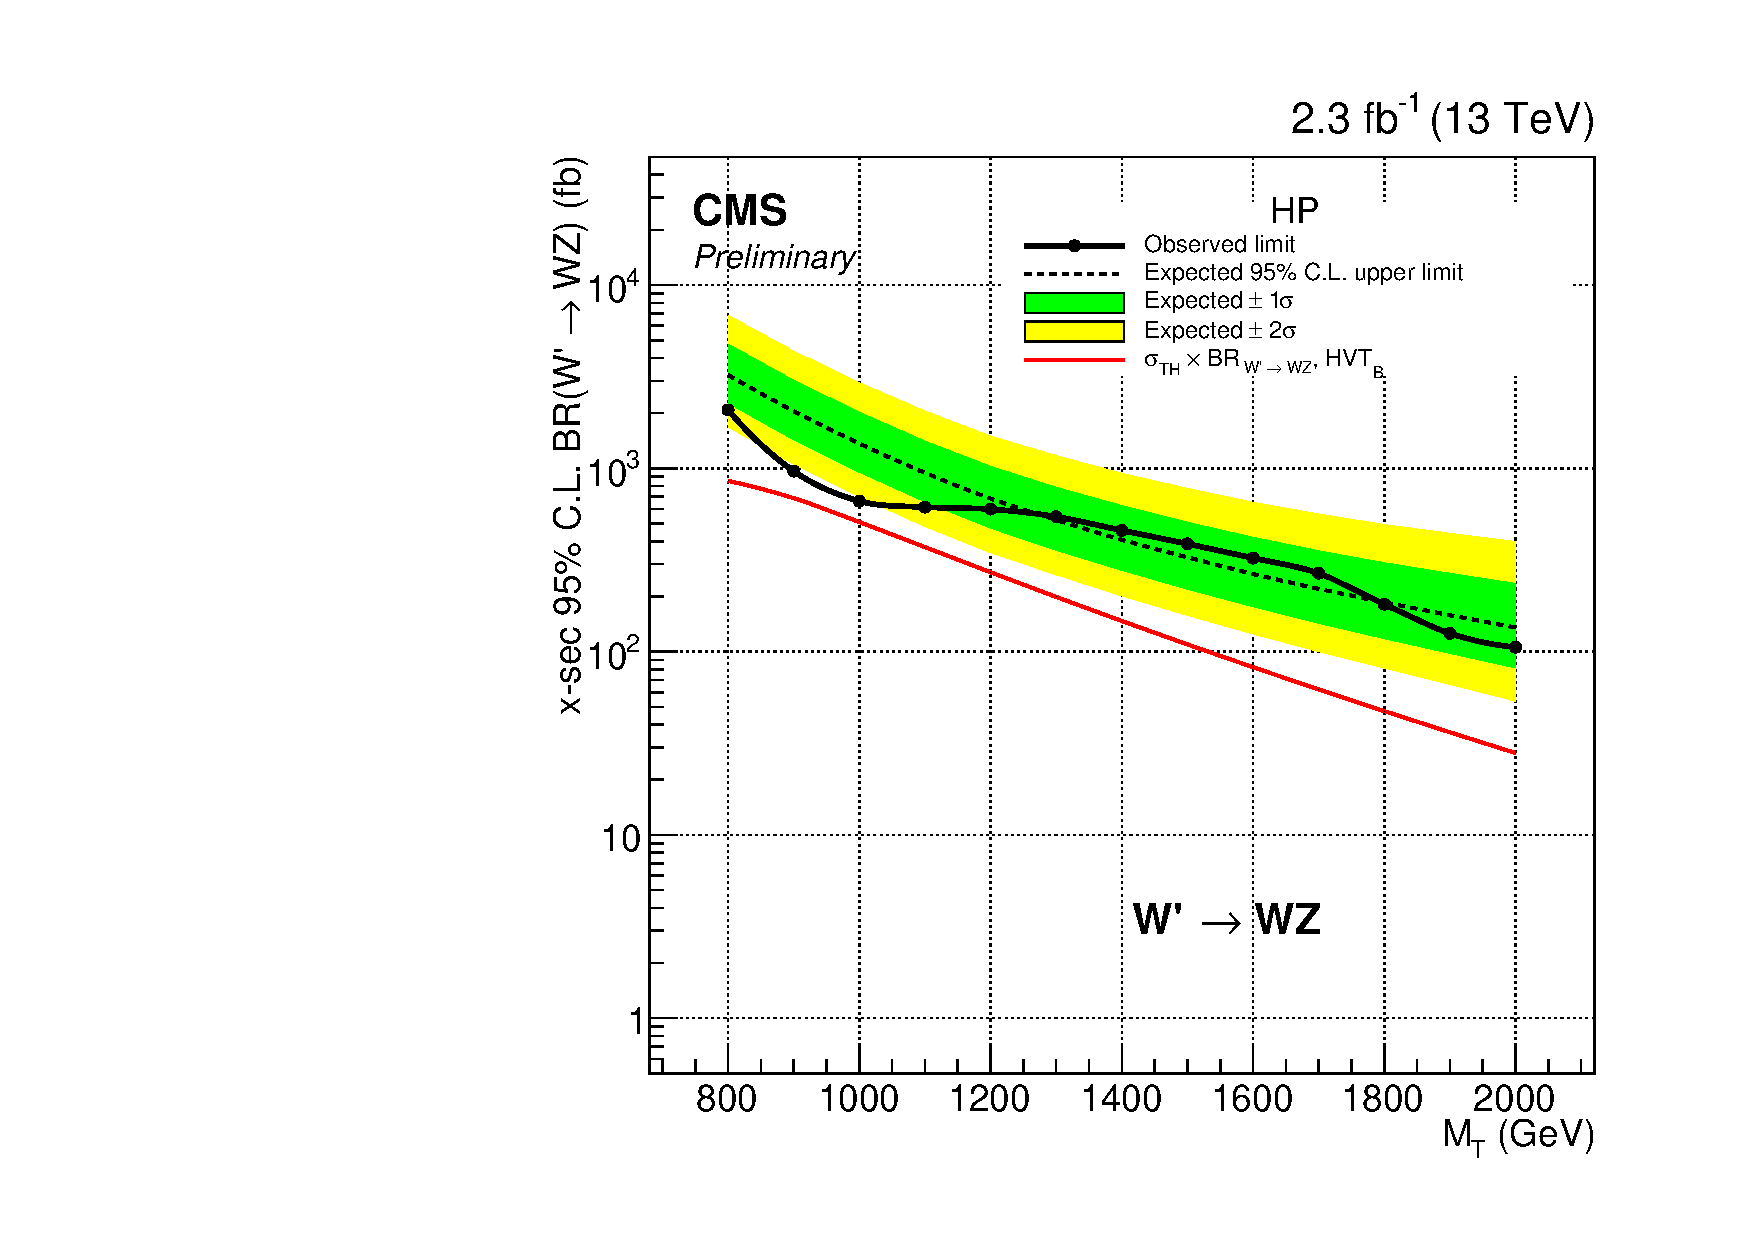
\includegraphics[width=200pt]{figuresARC/limits/limitWprimeHPUB.pdf} &
  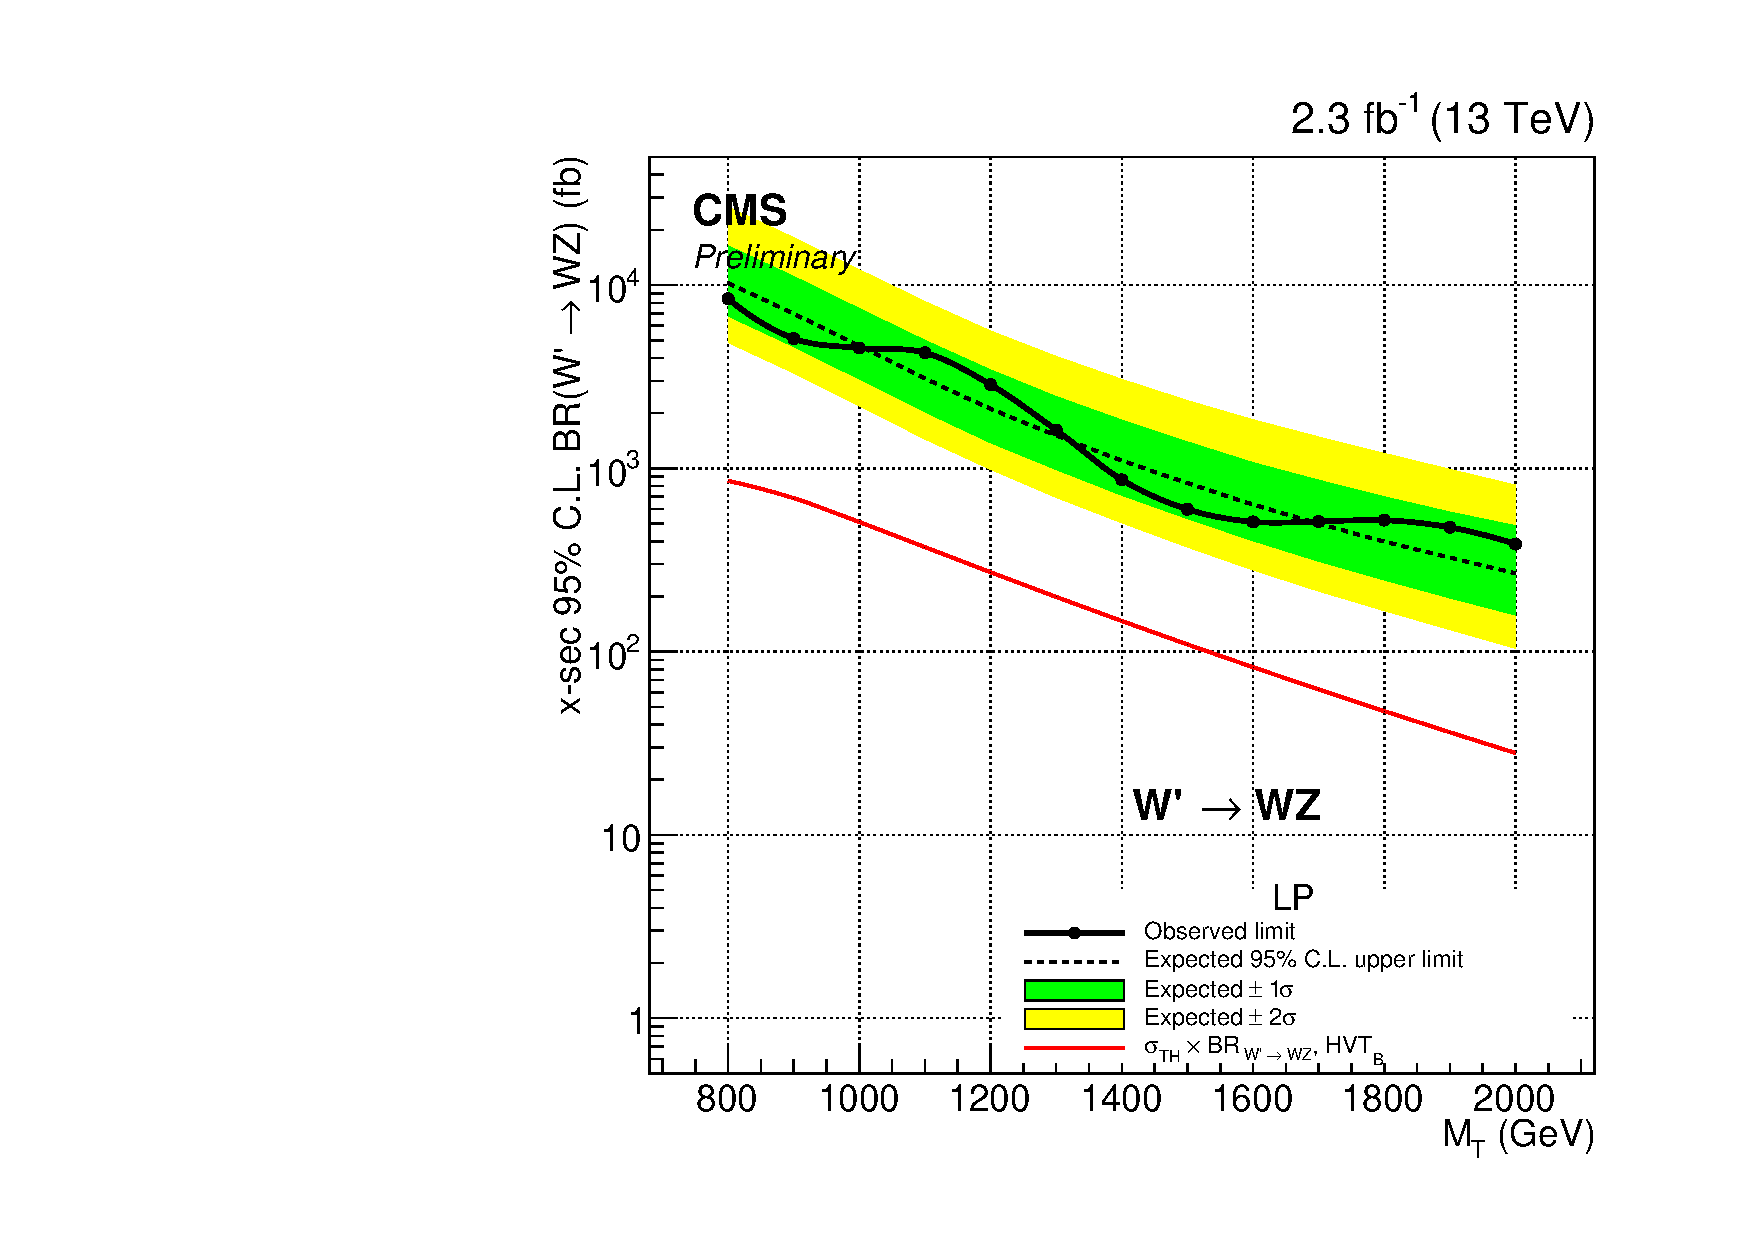
\includegraphics[width=200pt]{figuresARC/limits/limitWprimeLPUB.pdf}\\
\end{tabular}
\begin{center}
  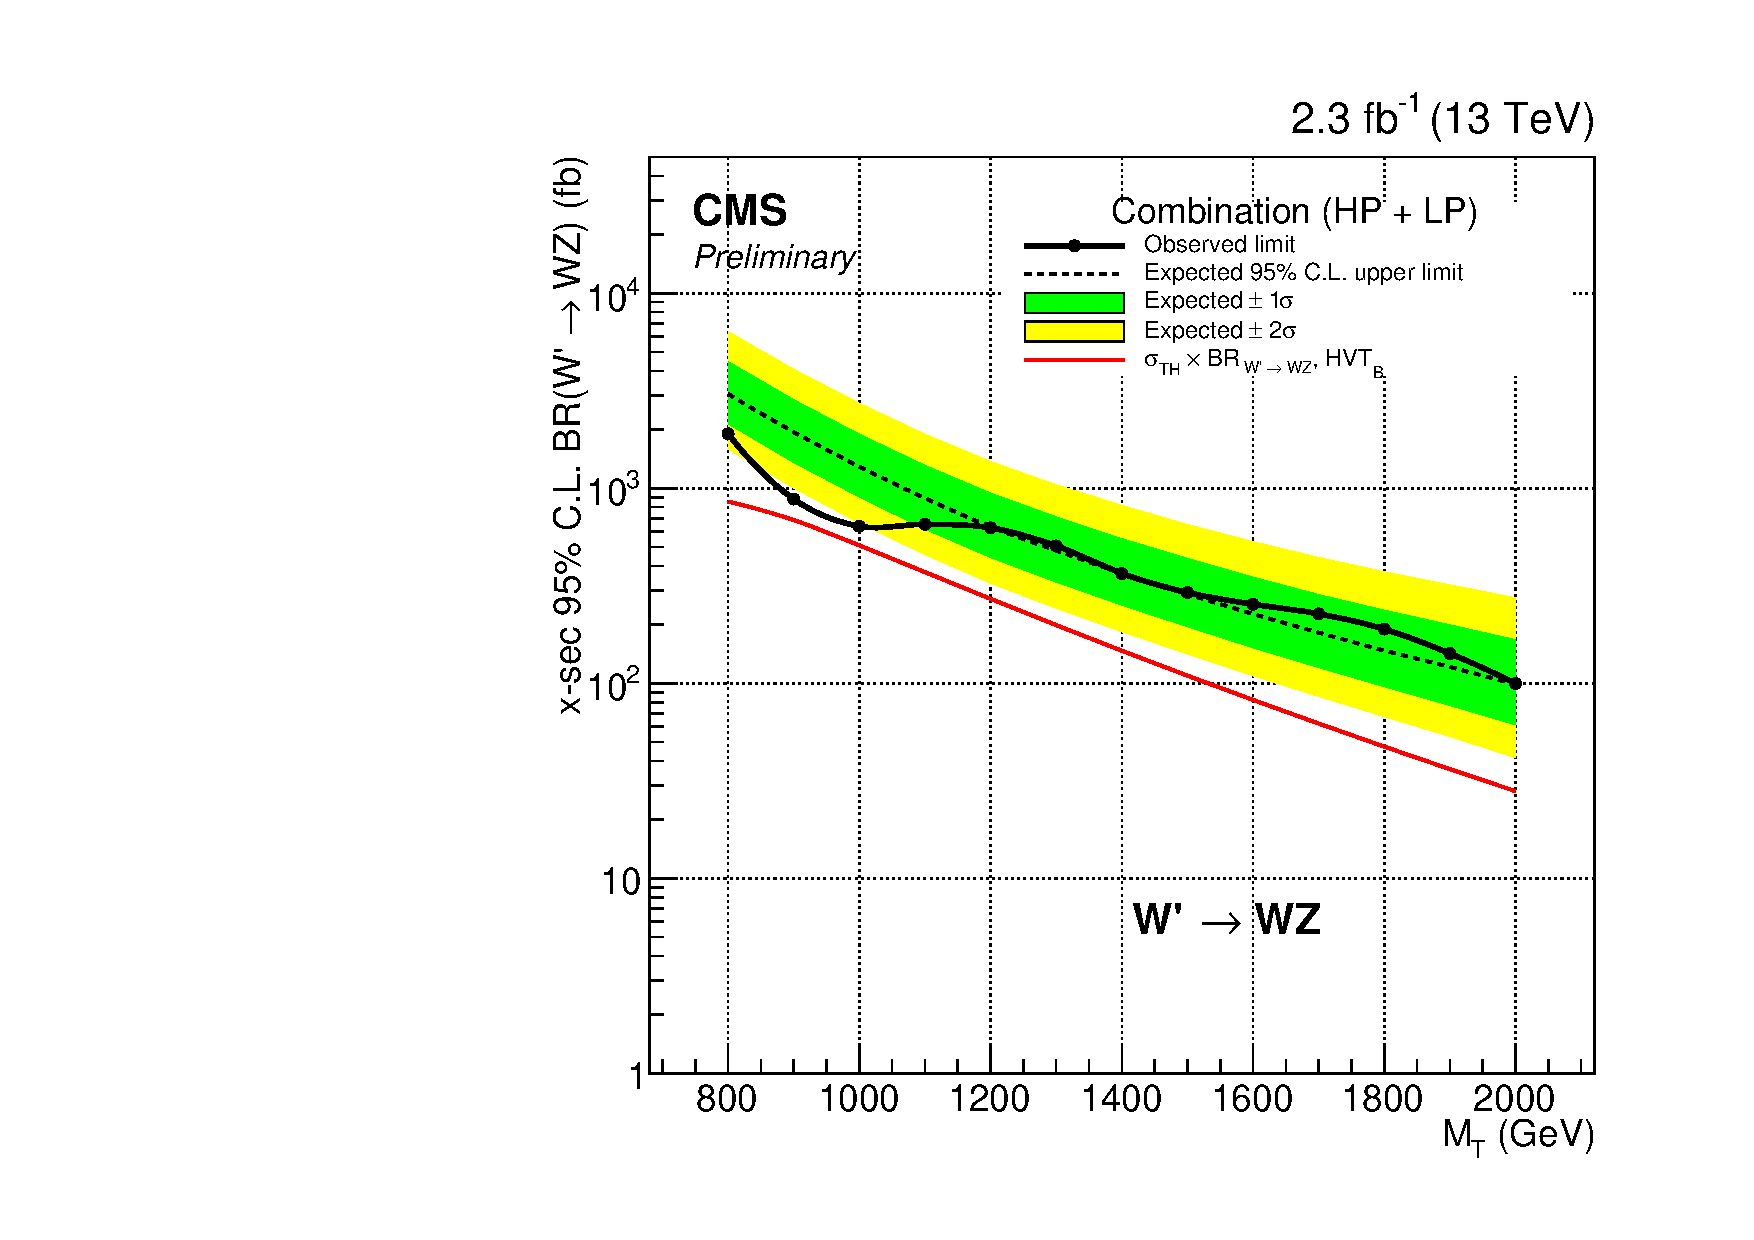
\includegraphics[width=250pt]{figuresARC/limits/limitWprimeNPUB.pdf}
\end{center}

\label{fig:limits2}
\end{figure}

\subsection{Crosscheck}

As a crosscheck of the asymptotic limit we run the fully frequentist CLs limit with the \emph{The HybridNew method}, which is the current recommended method by the LHC Higgs Combination Group.  
Figure \ref{fig:fulllimits} shows the comparison between the asymptotic and full CLs limit for the bulk graviton model in the HP and LP categories. 

\begin{figure}[!ht]
\caption{Observed and expected 95$\%$ CL upper limit on Bulk graviton production cross section times the branching fraction of $G_{bulk} \rightarrow  ZZ$ assuming an integrated luminosity of 2.318 fb$^{-1}$. In the figure we show the comparison between the full CLs method (blue) and the asymptotic limit (black). A good agreement is observed in the limit obtained for both methods.}
\begin{tabular}{cc}
  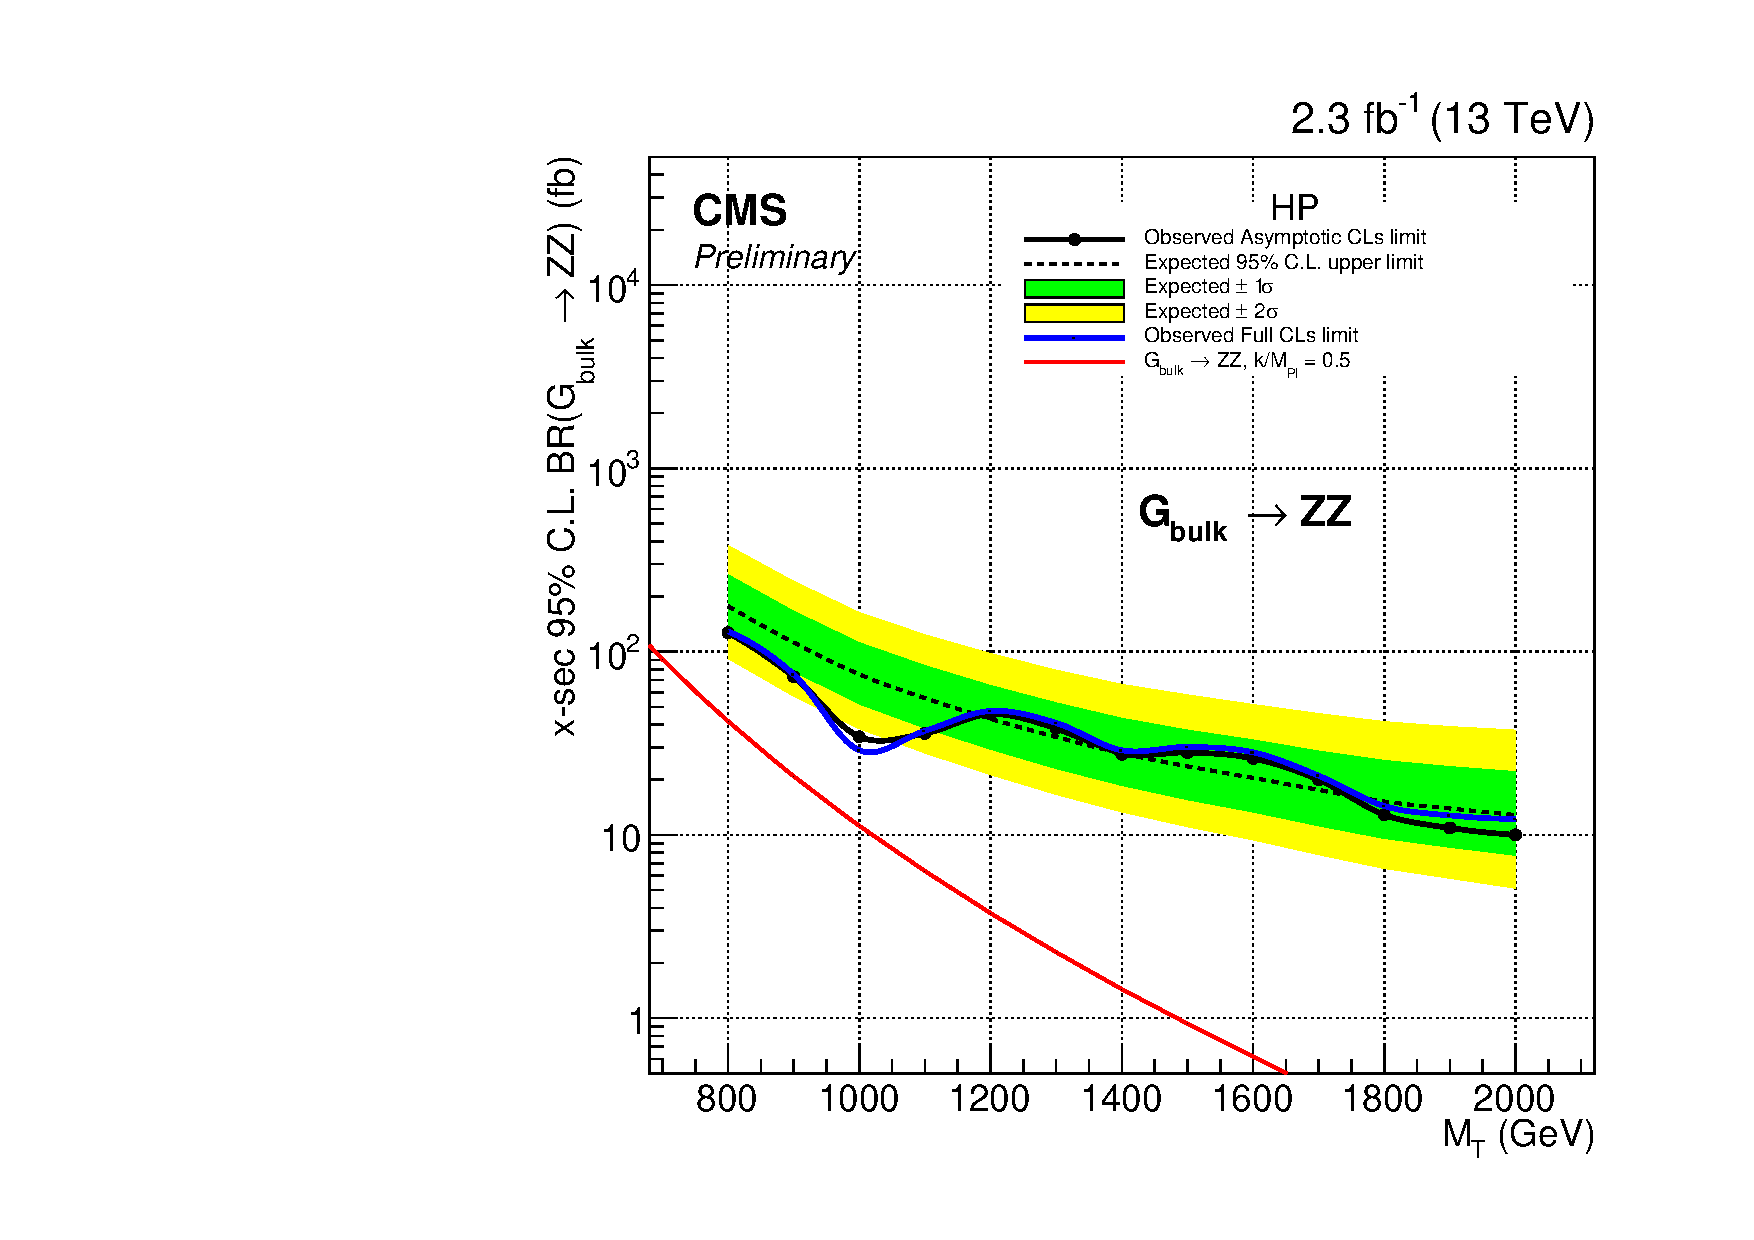
\includegraphics[width=200pt]{figuresARC/limits/fulllimitBulkGHP.pdf} &
  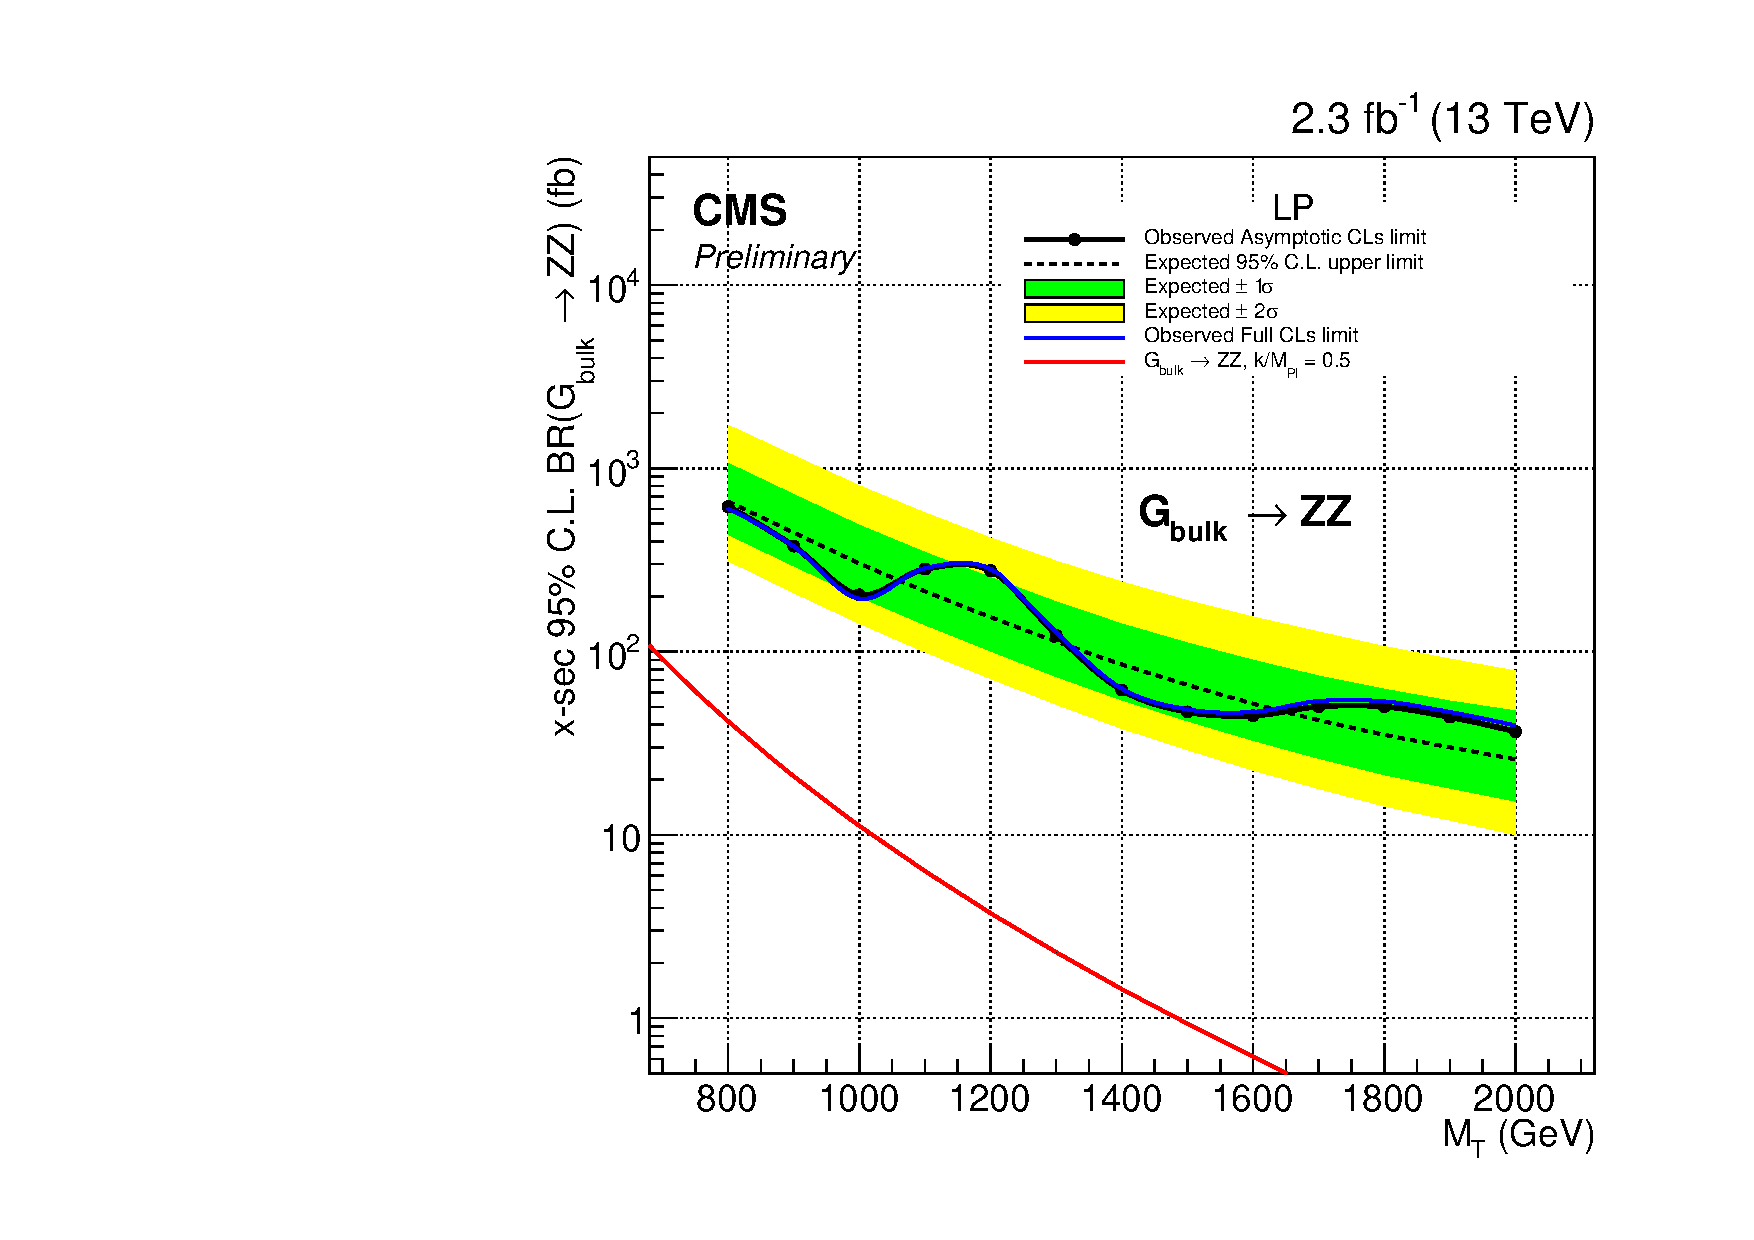
\includegraphics[width=200pt]{figuresARC/limits/limitBulkGFullLP.pdf}\\
\end{tabular}
\label{fig:fulllimits}
\end{figure}



